
\section{Fathi Rabbani / 1164074}
\subsection{Teori}
\begin{enumerate}
\item Matplotlib
\par Library yang ada pada pemrograman Python yang berguna untuk membuat data grafik yang berdimensi 2.

\item Membuat Sumbu X dan Y
\par membuat sumbu X dan Y pada penggunaan Library Matplotlib adalah dengan menjelaskan setiap detail data array yang dimiliki sebagai contohnya ada pada Code Berikut : 
\lstinputlisting[firstline=3, lastline=8]{src/chapter6/1164074/code.py}

\item Penggunaan Jenis Plot di Matplotlib
\par ada berbagai macam Jenis PLot yang ada pada Matplotlib, diantaranya adalah :
\begin{itemize}
\item \lstinputlisting[firstline=2, lastline=8, caption=Jenis Garis]{src/chapter6/1164074/code.py}
\item \lstinputlisting[firstline=11, lastline=13, caption=Jenis Titik]{src/chapter6/1164074/code.py}
\item \lstinputlisting[firstline=16, lastline=20, caption=Jenis Batang]{src/chapter6/1164074/code.py}
\item \lstinputlisting[firstline=23, lastline=33, caption=Jenis Pie]{src/chapter6/1164074/code.py}
\end{itemize}

\item Menggunakan Legend dan Label
\par Legend pada matplotlib digunakan untuk menunjukan penggunaan grafik yang ditampilkan. contohnya dapat dilihat pada code berikut : 
\lstinputlisting[firstline=36, lastline=38, caption=Code penggunaan Legend pada Matplotlib]{src/chapter6/1164074/code.py}

\par Label pada matplotlib digunakan untuk menambahkan data Text pada grafik agar mudah untuk dibaca.
\lstinputlisting[firstline=42, lastline=45, caption=Code penggunaan Label pada Matplotlib]{src/chapter6/1164074/code.py}

\item Fungsi subplot di Matplotlib
\par Fungsi yang digunakan untuk menambahkan beberapa diagram sekaligus dalam satu sintaks. contoh code dan penggunaannya dapat dilihat pada Code dan Gambar \ref{data1}
\lstinputlisting[firstline=48, lastline=74, caption= Code penggunaan Subplot pada Matplotlib]{src/chapter6/1164074/code.py}
\begin{figure} [!htbp]
	\centerline{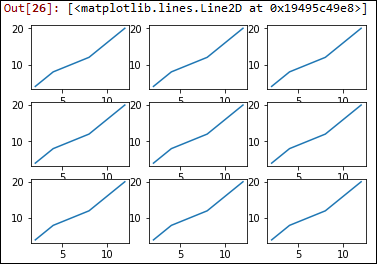
\includegraphics[width=0.5\textwidth]{figures/chapter6/1164074/1}}
	\caption{Penggunaan Subplot pada Matplotlib}
	\label{data1}
\end{figure}

\item Parameter Color
\par Penggunaan warna memiliki peran penting dalam membuat tampilan Grafik lebih menarik dan tidak membosankan, berikut ini adalah daftar penggunaan warna pada Matplotlib :

\begin{itemize}
	\item b : Untuk memberikan warna biru
	\item g : Untuk memberikan warna hijau
	\item r : Untuk memberikan warna merah
	\item c : Untuk memberikan warna biru muda
	\item m : Untuk memberikan warna pink
	\item y : Untuk memberikan warna kuning
	\item k : Untuk memberikan warna hitam
	\item w : Untuk memberikan warna putih
\end{itemize}


\item Cara kerja Fungsi hist
\par Fungsi Hist merupakan fungsi yang berguna untuk membuat data grafik Batang yang memiliki nilai banyak (Array). contoh Code dan penjelasanya dapat dilihat pada Gambar \ref{data2}
\lstinputlisting[firstline=77, lastline=81, caption= Code penggunaan Subplot pada Matplotlib]{src/chapter6/1164074/code.py}
\begin{figure} [!htbp]
	\centerline{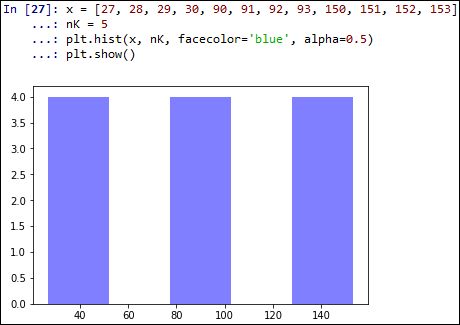
\includegraphics[width=0.5\textwidth]{figures/chapter6/1164074/2}}
	\caption{Hasil dari Penggunaan Hist dari Code tersebut}
	\label{data2}
\end{figure}

\item Keterangan Lebih tentang Parameter pada Fungsi Pie
\begin{itemize}
\item Labels
\par Isi dengan tipe data list dan tidak wajib untuk digunakan. Fungsi parameter labels untuk memberi label pada setiap pecahan data yang ada pada grafik pie yang ditampilkan.

\item Colors
\par Tipe data array atau sejenis dan tidak wajib untuk digunakan. Fungsi parameter colors untuk mengganti warna pada setiap pecahan yang ada. Jika tidak digunakan atau ditentukan, maka warna yang akan dipakai adalah warna yang aktif atau standar.
	
\item Startangle
\par Tipe data pecahan atau float, tidak wajib untuk digunakan. Fungsi parameter startangle adalah fungsi untuk memutar grafik agar berubah posisi dengan acuan yaitu angle awalan dari grafik pie.

	
\item Shadow
\par Bertipe data boolean dan tidak wajib digunakan. Fungsi parameter shadow digunakan untuk membuat bayangan pada bawah grafik pie yang ditampilkan. 
	
\item Explode
\par Bertipe data array atau sejenis dan tidak wajib digunakan. Fungsi parameter explode adalah menentukan radius untuk mengimbangi setiap pecahan pada grafik pie. Jika radius lebih dari 0 maka pecahan akan mulai menjauh dari pusat dan terlihat seperti keluar dari grafik lingkaran tersebut.

\item Autopct
\par Bertipe data string atau fungsi dan tidak wajib digunakan. Fungsi parameter autopct adalah memberi label pada irisan dengan labelnya berupa fungsi atau string. 
\end{itemize}

\item Check Plagiarisme

\begin{figure} [!htbp]
	\centerline{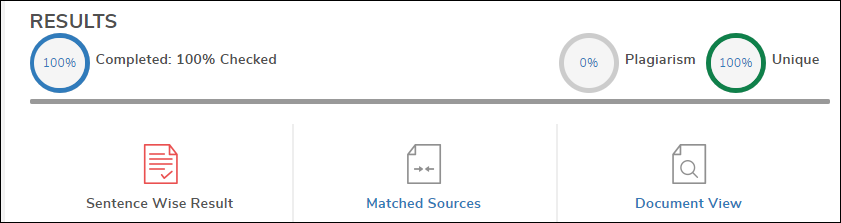
\includegraphics[width=0.5\textwidth]{figures/chapter6/1164074/3}}
	\caption{Hasil Check Data Plagiarisme}
	\label{data3}
\end{figure}
\end{enumerate}